\documentclass[12pt,a4paper]{article}
\usepackage[utf8]{inputenc}
\usepackage{amsmath}
\usepackage{amsfonts}
\usepackage{amssymb}
\usepackage{graphicx}
\usepackage[left=2cm,right=2cm,top=2cm,bottom=2cm]{geometry}
\author{leonardo}
\title{xplicación de circuitos con tiristores en convertidores CA-CD:}
\begin{document}
Un Tiristor es dispositivo semiconductor de cuatro capas de estructura pnpn con tres uniones pn tiene tres terminales: ánodo cátodo y compuerta. muestra el símbolo del tiristor y una sección recta de tres uniones pn. Los tiristores se fabrican por difusión.
Cuando el voltaje del ánodo se hace positivo con respecto al cátodo, las uniones J1 y J3 tienen polarización directa o positiva. La unión J2 tiene polarización inversa, y solo fluirá una pequeña corriente de fuga del ánodo al cátodo. Se dice entonces que el tiristor está en condición de bloqueo directo o en estado desactivado llamándose a la corriente fuga corriente de estado inactivo ID. Si el voltaje ánodo a cátodo VAK se incrementa a un valor lo suficientemente grande la unión J2 polarizada inversamente entrará en ruptura. Esto se conoce como ruptura por avalancha y el voltaje correspondiente se llama voltaje de ruptura directa VBO. Dado que las uniones J1 y J3 ya tienen polarización directa, habrá un movimiento libre de portadores a través de las tres uniones que provocará una gran corriente directa del ánodo. Se dice entonces que el dispositivo está en estado de conducción o activado.
\begin{center}
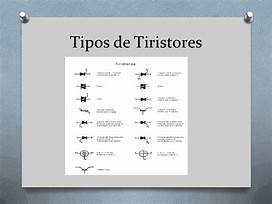
\includegraphics[width=10cm]{1.jpg}   
\end{center}
\begin{flushleft}
 La caída de voltaje se deberá a la caída óhmica de las cuatro capas y será pequeña, por lo común 1V. En el estado activo, la corriente del ánodo está limitada por una impedancia o una resistencia externa, RL, tal y como se muestra.
La corriente del ánodo debe ser mayor que un valor conocido como corriente de enganche IL, a fin de mantener la cantidad requerida de flujo de portadores a través de la unión; de lo contrario, al reducirse el voltaje del ánodo al cátodo, el dispositivo regresará a la condición de bloqueo. La corriente de enganche, IL, es la corriente del ánodo mínima requerida para mantener el tiristor en estado de conducción inmediatamente después de que ha sido activado y se ha retirado la señal de la compuerta. En la fig. 2b aparece una gráfica característica v-i común de un tiristor.  

\end{flushleft}
\begin{center}
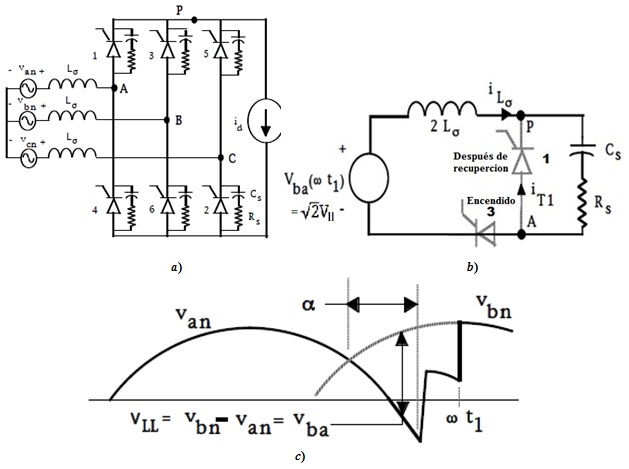
\includegraphics[width=10cm]{2.jpg} 
\end{center}
\begin{flushleft}
El SCR y la corriente Alterna:
Se usa principalmente para controlar la potencia que se entrega a una carga. (en el caso de la figura es un bombillo o foco
La fuente de voltaje puede ser de 110V c.a., 120V c.a., 240V c.a. , etc.
El circuito RC produce un corrimiento de la fase entre la tensión de entrada y la tensión en el condensador que es la que suministra la corriente a la compuerta del SCR. Puede verse que el voltaje en el condensador (en azul) está atrasado con respecto al voltaje de alimentación (en rojo) causando que el tiristor conduzca un poco después de que el tiristor tenga la alimentación necesaria para conducir.
Durante el ciclo negativo el tiristor se abre dejando de conducir. Si se modifica el valor de la resistencia, por ejemplo si utilizamos un potenciómetro, se modifica el desfase que hay entre las dos tensiones antes mencionadas ocasionando que el SCR se active en diferentes momentos antes de que se desactive por le ciclo negativo de la señal. y deje de conducir.

\end{flushleft}
\begin{center}
\includegraphics[scale=1]{../../Users/leo_2/Desktop/martinez.chavez.leonardo/tareas/Nueva carpeta/3.1.gif} 
\end{center}
\begin{flushleft}
Cómo funcionan los tiristores en un circuito:
 que utiliza realimentación interna para producir una conmutación.1 Los materiales de los que se compone son de tipo semiconductor, es decir, dependiendo de la temperatura a la que se encuentren pueden funcionar como aislantes o como conductores. Son dispositivos unidireccionales (SCR) o bidireccionales (Triac o DIAC). Se emplea generalmente para el control de potencia eléctrica.
Para los SCR el dispositivo consta de un ánodo y un cátodo, donde las uniones son de tipo P-N-P-N entre los mismos. Por tanto, se puede modelar como 2 transistores típicos P-N-P y N-P-N, por eso se dice también que el tiristor funciona con tensión realimentada. Se crean así 3 uniones (denominadas J1, J2, J3 respectivamente), el terminal de puerta está a la unión J2 (unión NP).
Algunas fuentes definen como sinónimos al tiristor y al rectificador controlado de silicio (SCR). Aunque en realidad la forma correcta es clasificar al SCR como un tipo de tiristor, a la par que los dispositivos DIAC y TRIAC.
Este elemento fue desarrollado por ingenieros de General Electric en los años 1960. Aunque un origen más remoto de este dispositivo lo encontramos en el SCR creado por William Shockley (premio Nobel de física en 1956) en 1950, el cual fue defendido y desarrollado en los laboratorios Bell en 1956. Gordon Hall lideró el desarrollo en Morgan Stanley para su posterior comercialización por parte de Frank W. "Bill" Gutzwiller, de General Electric.

\end{flushleft}
\end{document}